\chapter{Background Research}
%Background (10- 20 pages).  This should form the bulk of the interim report.
%You should consider that your objective here is to produce a near final
%version of the background section, as it will appear in your final report. 
% All of this material should be re-usable, so it is worth getting it right at
% this stage of the project.  The details of what to include can be found in
% the Project Report guidelines.

\section{Global Network properties}

Global network properties give an overall view of the network, but are usually
not detailed enough to capture complex topological characteristics. In the
following sections we will present a few key global properties such as degree
distribution, clustering coefficient and the average path length.

\subsection{Degree Distribution}

\begin{figure}[h]
  \centering
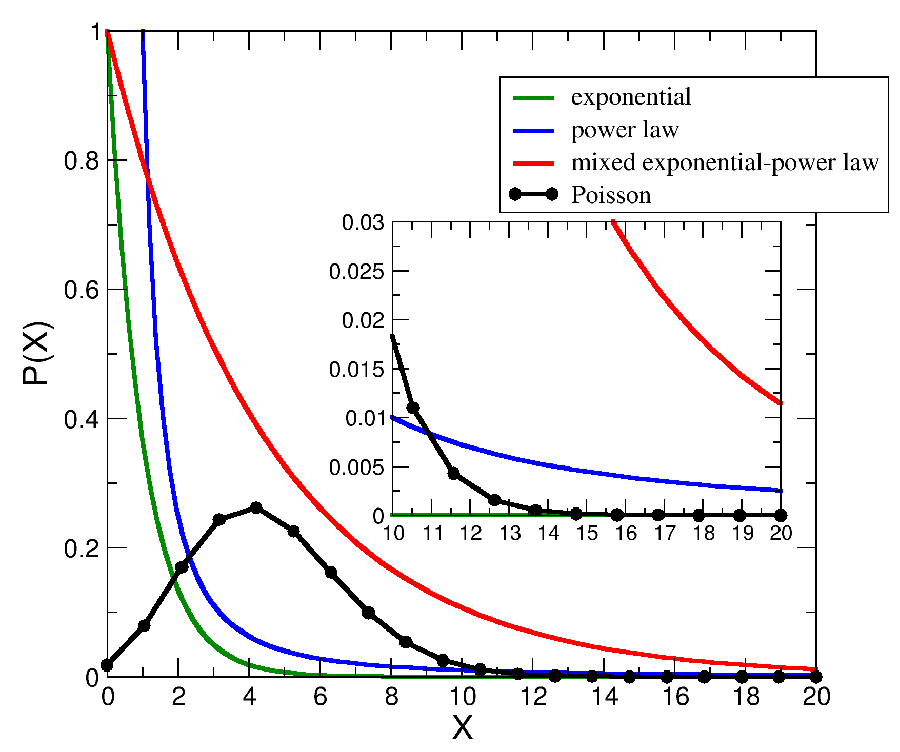
\includegraphics[scale=0.66]{images/deg_dist_all.png}
\caption{Graph depicting the most common classes of degree distributions:
Poisson, Power-law and Exponential.}
\label{fig:deg_dist_all}
\end{figure}

The degree distribution P(k) of a graph is the fraction of nodes in the network
having degree k. Several current classes exist, with the most commonly-used
ones being: Poison/Binomial, power-law and exponential (see fig.
\ref{fig:deg_dist_all}). A power-law degree distribution has a high number of
nodes with low degree and a very small
number of nodes with high degree, also called hub nodes.

Although many random graphs have a Poison degree distribution, it has been shown
that many real networks have a power-law degree distribution instead. Such
networks include the Internet, transportation networks, anatomical circulatory
networks, social networks and food webs.

\subsection{Clustering Coefficient}

\begin{figure}[h]
  \centering
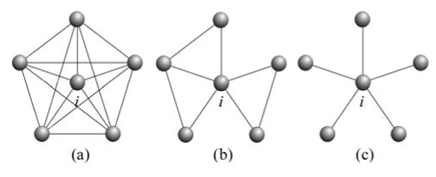
\includegraphics[scale=0.7]{images/clust_coeff.png}
\caption{The clustering coefficient intuitively describes how connected are
the neighbours of a particular node. In the above three scenarios, the
custering coefficient decreases from (a) to (c).
Image source\cite{costa2008complex}}
\label{fig:clust_coeff}
\end{figure}

The clustering coefficient is another important property of a graph that is used
for data analysis and comparisons. It measures the tendency of nodes to
cluster together. 

Watts and Strogatz defined the clustering
coefficient in the following manner: Consider a node n in a graph G that has $
k_n $ neighbours. The maximum number of edges between the neighbours of n is $
\frac{k_n (k_n - 1)}{2} $. Consider that only a fraction $ C_n $ of these edges
are present in the set of neighbours of n. $ C_n $ can also be viewed as the
probability of two neighbours of n being connected. This is then averaged
against all the nodes in the graph and the final clustering coefficient C of
graph G is obtained.  

It has been shown that real networks have a high clustering coefficient.
However, in the Erdos-Renyi graphs, the clustering coefficient is low when the
probability p of connecting two nodes is also low. This makes these
models unsuitable for modeling real data.

\subsection{Average path length}

The distance between two nodes is defined as the smalled number of links that
have to be traversed to get from one node to another. The average path length
of a network is therefore the average distance between any pair of two nodes. 

Real networks have been shown to exhibit a small average path length. In the
Erdos-Renyi graphs we have just mentioned, the average path length is large
when the probability p of connecting two edges is small, and it gets smaller as
p increases.





\section{Local Network properties}

Local network properties capture detailed information about a local region in
the network or even one single node. On the other hand, local properties cannot
give an overall description of the network. In the next few sections we will
present three main types of local metrics: Node centralities, \emph{Graphlet
Frequency Vector} and \emph{Graphlet Degree Vector}

\subsection{Node centralities}

Another commonly used property for measuring the importance of a node in a
network is the centrality. Several types of centralities include:
\begin{itemize}
 \item Degree centrality: Measures the number of links that connect with the
node. It is simply defined as the degree of the node.
 \item Betweenness centrality: Quantifies how many shortest paths pass through
the node
 \item Closeness centrality: Measure how close the node is to the other nodes
in the network.
% \item Eigenvector centrality: Assigns scores to the nodes based on the idea
%that connections to high-scoring nodes contribute more to the score of the node
%in question than connections to low-scoring nodes. This measure is used by
%Google's Page Rank algorithm\cite{jing2008pagerank}.
\end{itemize}

The Betweenness centrality of a node v is defined as the fraction of the
shortest paths from between two arbitrary nodes (i,j) that pass through v. It
can be formally defined as:

$$ B(v) = \sum_{s \ne v \ne t \in V}\frac{\sigma_{st}(v)}{\sigma_{st}}$$

, where $\sigma_{st}(v) $ is the number of shortest paths from s to t that pass
through node v, while $ \sigma_{st} $ is the total number of shortest paths
from s to t.

On the other hand, the Closeness centrality is based on another measure called
the \textbf{farness} of a node which is defined as the sum of its distances to
all the other nodes in the network. Therefore the closeness centrality is
defined as the inverse of the farness.

\subsection{Graphlets}

\begin{figure}[h]
  \centering
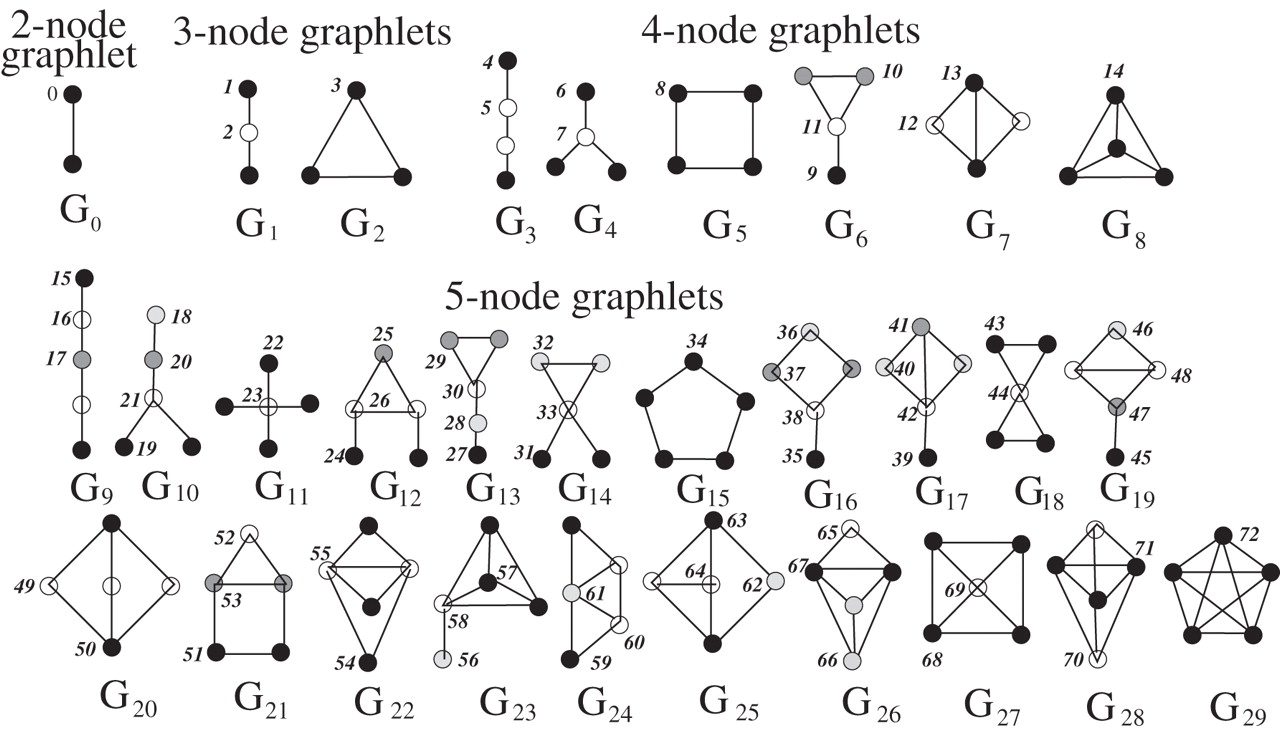
\includegraphics[scale=0.25]{images/graphlets.jpg}
\caption{Graphlets for sizes of 2, 3, 4 and 5 nodes. They are ordered in
groups according to the number of nodes and numbered from the least-dense to the
most dense. These are the graphlets that are generally counted when computing
the GDV and GCV metrics. Source:\cite{milenkoviae2008uncovering} }
\label{fig:graphlets}
\end{figure}

Graphlets are small connected non-isomorphic induced subgraphs of a graph. They
have been previously used by Natasa Przulj for developing some generalised
measures of computing local topological metrics such as the Graphlet
Distribution Vector (GDV).

For a given graph G, the \emph{Graphlet Frequency Vector} can be calculated by
counting the number of distinct graphlets of each type found in the network.
From here, we can normalise these against the total number of graphlets in G to
calculate the \emph{Relative Graphlets Frequency Vector}. This is thus defined
as:

\begin{equation}
 GFV(G) = \left(F_1(G), F_2(G), ... F_{29}(G)\right)
\end{equation}

where:

$$ F_i(G) = -log\left(\frac{G_i}{\sum_{i=1}^{n}G_i}\right) $$

\begin{figure}[h]
  \centering
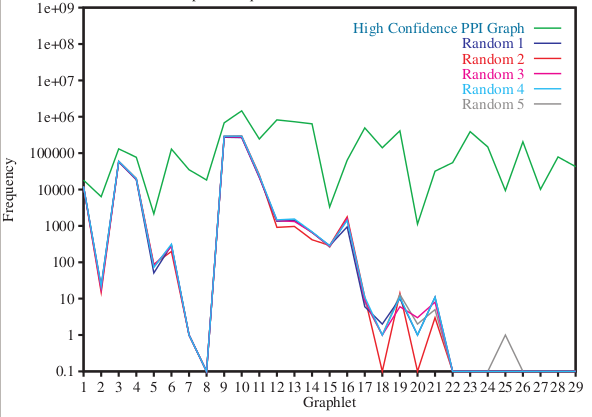
\includegraphics[scale=0.7]{images/gdv-er-interactome.png}
\caption{Example of a Graphlet degree vector for the PPI network of yeast
\emph{Saccharomyces cerevisiae}. As one can see from the graph, the GDV
signature of the real network is considerably different from the ones of the
random networks. The random networks have been generated using the Erdos-Renyi
method. Source: \cite{prvzulj2004modeling}}
\label{fig:gdv_er}
\end{figure}

\subsection{Relative Graphlet Frequency Distance}

Using the Graphlet frequencies that have been previously defined, we can now
compute a measure of disparity between two graphs by taking pairs of
graphlet frequencies for each type and then summing their absolute difference.
This is called the \emph{Relative Graphlet Frequency Distance} (RGFD). More
formally, if we consider two graphs G and H and we denote \(F_i(G)\) and
\(F_i(H)\) to be the frequency of the i-th graphlet in G and H, then we
compute the RGFD as:

\begin{equation}
 D = \sum_{i=1}^{n}| G_i - H_i |
\end{equation}


\subsection{Graphlet Degree Vectors}

The Degree Distribution of a network calculates the number of nodes touching k
edges for each value of k. However, we can generalise this concept by looking
at the 73 automorphism orbits (see fig \ref{fig:graphlets}) and counting the
number of nodes that touch a particular graphlet at a particular orbit. Finally,
we get a spectrum of 73 \emph{Graphlet Degree Distributions (GDDs)} measuring
local properties of a network. 


\subsection{GDD Agreement}

We are now trying to compare the spectra of 73 Graphlet Degree Distributions
belonging to a graph G to the ones corresponding to another graph H. There
might be several ways to perform this, but we will present the method used by
N. Przulj in 2006\cite{prvzulj2007biological}. 

Let G be a graph and let \( d_G^j(k) \) be a sample distribution of the
number of nodes in G touching orbit j (j = 1-73) k times. Therefore, \( d_G^j
\) represents the j-th graphlet degree distribution (GDD). We scale \( d_G^j
\) as:

$$ S_G^j(k) = \frac{d_G^j(k)}{k} $$

in order to increase the contribution of the higher degrees. The reason for 
doing this is because most of the information is retained in the lower
degrees, whereas the high degrees mostly contain
noise\cite{prvzulj2007biological}. Afterwards, the distribution is normalised
against its total area:

$$ T_G^j = \sum_{k=1}^{\infty}S_G^j(k) $$

giving the normalised distribution:

$$ N_G^j(k) = \frac{S_G^j(k)}{T_G^j}. $$

The reason why we are normalising the distribution is because a large
network would have more nodes that potentially touch orbit j and therefore a
large area under the curve. Normalising it would make large and small
biological networks comparable in terms of their GDD. Finally, for two graphs G
and H and an orbit j, we define the distance \( D^j(G,H) \) between their
normalized j-th distributions as:

$$ D^j(G,H) = \sqrt{\sum_{k=1}^{\infty}[N_G^j(k) - N_H^j(k)]^2} $$

The distance \( D^j(G,H) \) is between 0 and 1, where 0 means that G and H have
the same GDD for automorphism orbit j. Now, we invert the this distance in
order to get the \emph{j-th GDD agreement}:

$$ A^j(G, H) = 1 - D^j(G,H)$$

where \(j \in {0,1,...,72}\). Finally, the GDD agreement between the two
networks G and H is the arithmetic mean of \( A^j(G,H) \) over all j:

$$ A(G,H) = \frac{1}{73}\sum_{j=0}^{72}A^j(G,H) $$



\section{Random graphs}

Random graphs are graphs that are usually generated using a random process.
They are used in data analysis for comparing or aligning them against
real networks. They can clarify the behaviour of
real-world networks, such as the world-wide web or protein-protein interaction
networks. Random graph models have been successfully used in various biological
settings, such as: Network motifs\cite{milo2002network}, De-noising of
protein-protein interaction network data\cite{kuchaiev2009geometric} or Guiding
biological experiments\cite{lappe2003unraveling}.


\subsection{Erdos-Renyi graphs}

The work on random graphs started from the influential publications of
Erdos and Renyi in the 1950s and 1960s, while Edgar Gilbert published a similar
model later on. Erdos and Renyi described the \(\mathbf{G_{n,m}}\)
model\cite{erdHos1959random}, while Gilbert described the \(\mathbf{G_{n,p}}\)
model\cite{gilbert1959random}. The two methods they described were as
follows: 
\begin{itemize}
 \item \(\mathbf{G_{n,p}}\):We start with n disconnected nodes and given
probability p. We then go through every pair of nodes and connect them with
probability p.

 \item \(\mathbf{G_{n,m}}\):We start with n disconnected nodes and a target of
m edges. Afterwards, we randomly select m pairs of nodes and connect them.
\end{itemize}

Although these networks are very easy to generate, it was later found
that real networks have a different structure that is different from the
Erdos-Renyi graphs. More precisely, they have a different degree distribution
and a low clustering coefficient. For the Erdos-Renyi $ G_{n,p} $ graph, the
degree distribution is binomial:

\begin{equation}
 P(k) = {n-1 \choose k} p^k (1-p)^{n-1-k}
\end{equation}

which can be approximated with a Poisson distribution for a large $n$:

\begin{equation}
 P(k) = \frac{z^k * e^{-z}}{k!}
\end{equation}

\begin{figure}[h]
  \centering
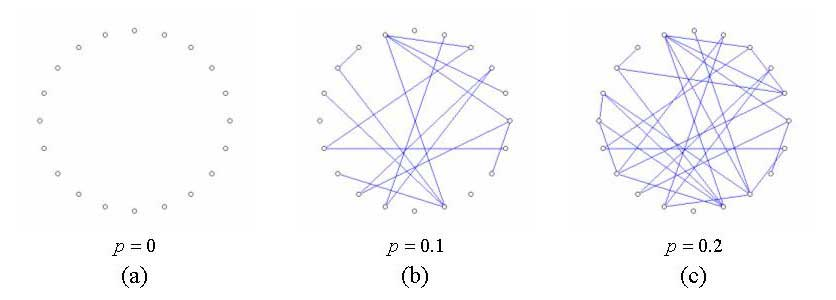
\includegraphics[scale=0.5]{images/erdos-renyi.jpg}
\caption{Example of three an Erdos-Renyi random graphs generated using the
\(G_{n,p}\) method. The three different graphs differ according to the
probability p of connecting one pair of nodes: (a) The graph is completely
disconnected. (b) The graph is sparsely connected as the probability p is low
(c) The graph becomes more dense as p increases to 0.2.
Source:\cite{erd6s1960evolution}}
\label{fig:erdos_renyi_graphs}
\end{figure}

\subsection{Erdos-Renyi with the degree distribution of a real network}

As we have previously seen, the degree distribution of an Erdos-Renyi graph
does not match real data. We will now present a method for constructing an
Erdos-Renyi network that preserves the degree distribution of a real network. 

We start with $n$ disconnected nodes. Each node is assigned a number of stubs 
according to the degree distribution of the real network that is being
modelled. A stub is simply a slot belonging to a particular node from where an edge can 
be connected. Afterwards, edges are created only between random pairs of nodes with
available stubs. After an edge is created, the number of stubs left available
at the nodes that were just connected is decreased by one. Moreover, edges
between one node and itself are not allowed.

This "stubs method" allows us to create ER (Erdos-Renyi) networks that have a power-law
degree distribution and a small average path length. Unfortunately, they still
have a low clustering coefficient.

\subsection{Scale-free networks}

\begin{figure}
  \centering
  \begin{subfigure}[b]{0.4\textwidth}
    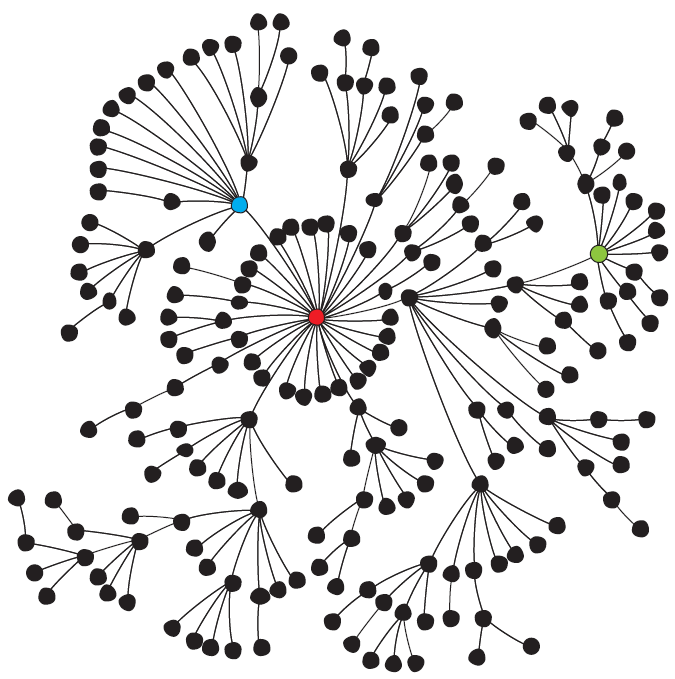
\includegraphics[width=\textwidth]{images/scale-free-network.png}
    \caption{Example of a scale-free network. Note the large
    number of nodes of small degree at the periphery of the network, while the
    number of hub nodes is very small.}
    \label{fig:scale_free_network}  
  \end{subfigure}
  ~ %add desired spacing between images, e. g. ~, \quad, \qquad etc.
    %(or a blank line to force the subfigure onto a new line)
  \begin{subfigure}[b]{0.5\textwidth}
    \centering
    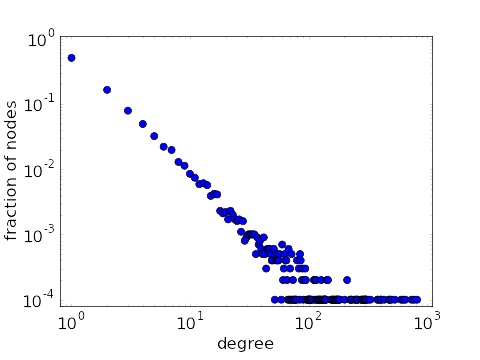
\includegraphics[width=\textwidth]{images/deg_dist_scale_free.png}
    \caption{The degree distribution of a scale-free network. As the degree of
the nodes gets larger, the fraction of nodes decreases exponentially. Notice
the logarithmic scale on the Y axis. It has been observed that many real
networks exhibit a scale free distribution.}
    \label{fig:degree_distribution}    
   \end{subfigure}
   \caption{Scale-free networks and degree distribution}
   \label{fig:scale_free} 
\end{figure}


Scale free networks are networks that normally exhibit a power-law degree
distribution (see fig \ref{fig:scale_free}). That is, $ P(k) = k^{-\gamma} $,
where $P(k)$ is the fraction of
nodes having degree $k$. It is currently believed that many networks such as the
world-wide web, social networks or biological networks exhibit a power-law
degree distribution.

\subsubsection{Barabasi-Albert model}

There are several proposed ways in which scale-free networks can be
generated. The Barabasi-Albert model is one such technique that uses the
\emph{preferential attachment} mechanism, with which nodes of high degree have
a high probability of receiving even more connections. 

In order to construct a network using the Barabasi-Albert method, we start with
an initial connected network of $ m_0  $ nodes. New nodes are consecutively
added to the network one at a time. Each one of them is connected to $ m <= m_0 
$ target nodes with a probability that is proportional to the degree of the
target nodes. Formally, the probability $ p_i $ that the new node is connected
to node i is:

\begin{equation}
 p_i = \frac{k_i}{\sum_{j}k_j}
\end{equation}

where $ k_i $ is the degree of node $i$, while the sum is over all the
nodes $j$ that already existed in the network when the new node is added. Because
of the preferential mechanism, heavily linked nodes (also called hub nodes)
tend to quickly accumulate links, whereas nodes with a low degree are unlikely
to be chosen. It has also been shown that the starting network heavily
influences the properties of the resulting network\cite{hormozdiari2007not}.

\subsection{Geometric graphs}

Geometric graphs are generated by fixing a certain metric space and using
metrics such as geometric distance or radius to connect edges together. A
metric space is a space that has a distance norm associated to it, such as: the
Euclidean distance, Chessboard distance or Manhattan distance.

Such a network is generated in the following manner:
\begin{enumerate}
 \item Choose a metric space and place nodes within the space using a uniform
random distribution.
 \item If any nodes are within distance $d$ from each other, then connect them
with an edge.
 \item $d$ needs to be chosen so that the end number of edges matches the network
that is modeled.
\end{enumerate}

\begin{figure}
  \centering
  \begin{subfigure}[b]{0.33\textwidth}
    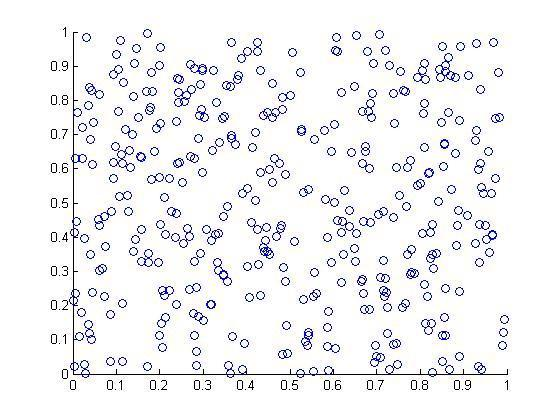
\includegraphics[width=\textwidth]{images/geometric1.png}
    \caption{}
    \label{fig:geo1}  
  \end{subfigure}
  ~ %add desired spacing between images, e. g. ~, \quad, \qquad etc.
    %(or a blank line to force the subfigure onto a new line)
  \begin{subfigure}[b]{0.33\textwidth}
    \centering
    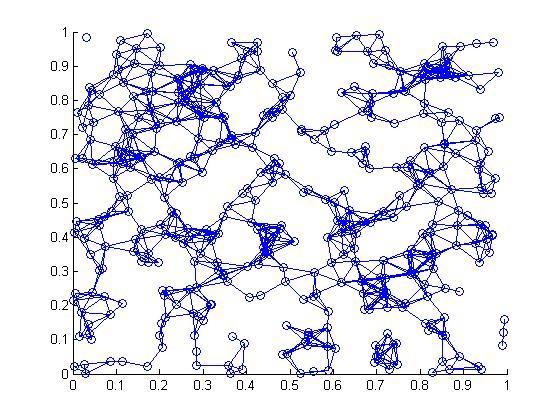
\includegraphics[width=\textwidth]{images/geometric2.png}
    \caption{}
    \label{fig:geo2}    
   \end{subfigure}
    ~ %add desired spacing between images, e. g. ~, \quad, \qquad etc.
    %(or a blank line to force the subfigure onto a new line)
  \begin{subfigure}[b]{0.33\textwidth}
    \centering
    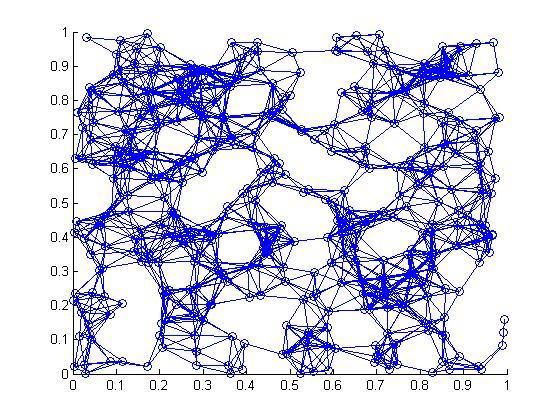
\includegraphics[width=\textwidth]{images/geometric3.png}
    \caption{}
    \label{fig:geo3}    
   \end{subfigure}
    ~ %add desired spacing between images, e. g. ~, \quad, \qquad etc.
    %(or a blank line to force the subfigure onto a new line)
  \begin{subfigure}[b]{0.33\textwidth}
    \centering
    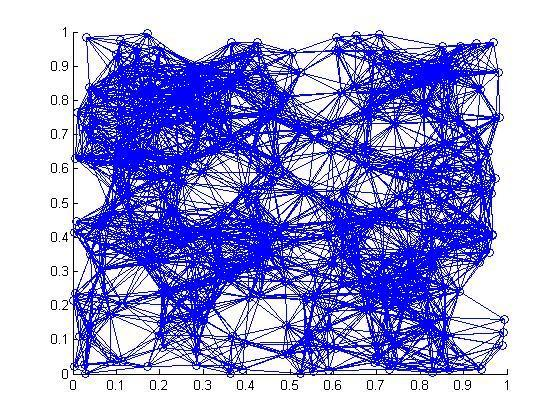
\includegraphics[width=\textwidth]{images/geometric5.png}
    \caption{}
    \label{fig:geo4}    
   \end{subfigure}
   \caption{Geometric networks for increasing distance d starting from
0. When $d = 0$ in graph (a), the nodes are all disconnected from each other. As
$d$ increses in graphs (b - d), the number of connections in the network also
increases proportionally. When using a Geometric network to model a real
network, one would normally use a value of $d$ that would yield a similar number
of edges as the real network.}
   \label{fig:geometric} 
\end{figure}

\subsection{Stickiness index-based graphs}

Przulj et al. have proposed in 2006 a simple random
graph model that inserts a connection according to the degree, or 'stickiness',
of the nodes involved\cite{prvzulj2006modelling}. This model has been inspired
from analysing protein-protein interactions and is based on two assumptions:
\begin{enumerate}
 \item A node having a high degree, or stickiness, implies that the
corresponding protein has many binding domains and/or its binding domains are
commonly involved in interactions.

 \item A pair of proteins is more likely to interact, or share complementary
binding domains, if they both have a high degree/stickiness. On the other hand,
if one or both of them have a low stickiness index, they are less likely to
interact. Thus, the product of their stickiness values can be used as the
probability of connecting the nodes.
\end{enumerate}

Considering the above assumptions, a stickiness based random graph can be
constructed as follows:
\begin{enumerate}
 \item We start with a network of $n$ nodes each having a degree $ deg_i $
sampled from a degree distribution of our choice
 \item For each node $i$, we compute the stickiness index $
\theta_i=deg_i/\sqrt{\sum_{j=1}^{N}deg_j}. $ Note that $ 0 \leq \theta_i \leq 1$
 \item For each pair of nodes $(i,j)$, we connect them with probability $
\theta_i \theta_j $
\end{enumerate}


\subsection{Random graph Comparisons}

As can be clearly seen in table \ref{tab:network_comparison}, real networks
normally have a power-law degree distribution, high clustering coefficient and
a small average path length. In terms of degree distribution, only Erdos-Renyi
(with a custom degree distribution), Barabasi-Albert and Stickiness-based
random networks have a power-law degree distribution, like that found in real
networks. However, it must be noted that although most of the real networks
have a power-law degree distribution, this is still a matter of research. For
example, it has been shown that Interactome network can be better modeled with
a Geometric network, instead of a Scale-free network having a power-law degree
distribution\cite{prvzulj2004modeling}.

On the other hand, only the Geometric and the Stickiness based models have a
high clustering coefficient. This is again something which has been observed in
most of the real networks such as social networks or biological networks.
Finally, most of the networks have a small average path length. It can
therefore be noted that the Stickiness based network is was the most successful
at modeling real-world phenomena with respect to these three properties.
However, there might be other network properties, such as various node
centralities\cite{newman2009networks} or \emph{Relative Graphlet Frequency
Agreement}, with can also be employed to
assess the suitability of the random networks. Identifying which of these 
properties can best compare various types of networks is still an open problem in
Network Analysis.

\definecolor{blue3}{HTML}{86B7FC} % med blue
\definecolor{blue1}{HTML}{B5F1FF} % light blue
\definecolor{blue2}{HTML}{E0F9FF} % very light blue

\definecolor{darkgreen}{HTML}{000000} % dark green

\rowcolors{1}{blue1}{blue2}

\begin{table}
  \centering
  Comparison of real networks versus randomly generated networks 
  \begin{tabular}{ | l | c | c | c |  }
    \hline
    \cellcolor{blue3} Model & \cellcolor{blue3} Degree Distribution &
  \cellcolor{blue3} Clustering coefficient & \cellcolor{blue3} Average path
length \\
    \hline
    Real networks & \textcolor{darkgreen}{Power-law} &
  \textcolor{darkgreen}{High} & \textcolor{darkgreen}{Small}\\
    \hline
    Erdos-Renyi & \textcolor{red}{Poisson} & \textcolor{red}{Low} &
  \textcolor{red}{Large (for small p)} \\
    \hline
    Erdos-Renyi - DD & \textcolor{darkgreen}{Power-law} &
  \textcolor{red}{Low} & \textcolor{darkgreen}{Small} \\
    \hline
    Barabasi-Albert & \textcolor{darkgreen}{Power-law} &
  \textcolor{red}{Low} & \textcolor{darkgreen}{Small} \\
    \hline
    Geometric (uniform) & \textcolor{red}{Poisson} &
  \textcolor{darkgreen}{High} & \textcolor{darkgreen}{Small} \\
    \hline
    Stickiness based & \textcolor{darkgreen}{Power-law} &
  \textcolor{darkgreen}{High} & \textcolor{darkgreen}{Small} \\
    \hline
  \end{tabular}
  \caption{As one can observe from the table above, the early models
such as Erdos-Renyi are not suitable for modeling real networks according to
these metrics. On the other hand, other random models such as the Stickiness
based satisfy all the three criteria. Nonetheless, it might still be different
from real networks with regards to other properties, such as node
centralities\cite{newman2009networks}. }
  \label{tab:network_comparison}
\end{table}

\section{Measuring Correlation}

In previous sections we have presented two main methods for calculating
how closely two GDV vectors match: \emph{Relative Graphlet Frequency Distance}
 and \emph{Graphlet Degree Distribution Agreement}. Although these are quite
efficient when comparing two networks, we can devise a better metric by using
some statistical techniques and a correlation coefficient such as \emph{Pearson's
product-movement correlation coefficient} or \emph{Spearman's rank correlation
coefficient}.

\subsection{Pearson's product-movement correlation coefficient}

Given two random variables $X$ and $Y$ from a population, \emph{Pearson's
correlation coefficient} or sometimes called \emph{Pearson's population
correlation coefficient} is defined as the ratio between the covariance of $X$
and $Y$ and the product of their standard deviation. It was introduced by Karl
Pearson and it is based on a similar idea by Francis Galton in the
1880\cite{stigler1989francis}\cite{lee1988thirteen}. It is formally defined as:

$$ \rho_{X,Y} = \frac{cov(X,Y)}{\sigma_X\sigma_Y} =
\frac{E[X-\mu_X]E[Y-\mu_Y]}{\sigma_X\sigma_Y}$$

,where $ \rho_{X,Y} $ is Pearson's correlation coefficient between random
variables $X$ and $Y$, $ cov(X,Y) $ is the covariance, while $\sigma_X $ and $ \mu_X
$ are the standard deviation and the expectation of $X$.

Pearson's correlation coefficient can also be applied to a sample from a given
population, in which case it is called the \emph{sample Pearson's correlation
coefficient} and is commonly denoted by $r$. This can be calculated by using
sample estimators for the covariance and standard deviation in the formula
above. The formula for the \emph{sample Pearson's correlation
coefficient} is:

\begin{equation}
\label{pears_corr}
 r = \frac{\sum_{i=1}^{n}(X_i - \bar{X})(Y_i -
\bar{Y})}{\sqrt{\sum_{i=1}^{n}\left(X_i -
\bar{X}\right)^2}\sqrt{\sum_{i=1}^{n}\left(Y_i -
\bar{Y}\right)^2}} 
\end{equation}

The values of both the sample and the population variants of Pearson's
correlation coefficients are between -1 and 1. Sample data points that have 
exactly 1 or -1 as their correlation coefficient will lie on a straight line.
Moreover, Pearson's correlation coefficient is symmetric, because: 

$$ corr(X,Y) = corr(Y,X) $$

where corr(X,Y) is defined as the correlation between random variables $X$ and $Y$.

\subsubsection{Pearson's distance}

Given a correlation coefficient $ \rho_{X,Y} $, a distance metric
called the Pearson's distance can be derived as
follows\cite{fulekar2009bioinformatics}:

$$ d_{X,Y} = 1- \rho_{X,Y} $$

It should be noted that because Pearson's correlation coefficient lies between
-1 and 1, then the Pearson's distance will have a value between 0 and 2.

\subsubsection{Interpretation}

Several researchers have provided guidelines into how
to interpret the size of the correlation coefficient\cite{cohen1988statistical} 
(equation \ref{pears_corr}).
However, interpretation is highly dependent on the context of the problem. For
example, a correlation of 0.8 might be low if one verifies physical laws using
measurements made with high-precision instruments, but it might be considered
high when applied to the analysis of social networks, because of other hidden
factors.

\subsection{Spearman's rank correlation coefficient}


\begin{figure}[h]
  \centering
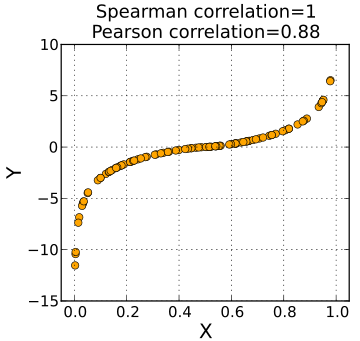
\includegraphics[scale=0.6]{images/spearman1.png}
\caption{Spearman's correlation coefficient is measuring how well the
dependence between two variables can be modeled
using a monotonic function. A Spearman's correlation of 1 can result even
when the data points are not linear, as long as they are monotonically related.
Source:\cite{spearman2009Wiki}}
\label{fig:spearman1}
\end{figure}


\begin{figure}[h]
  \centering
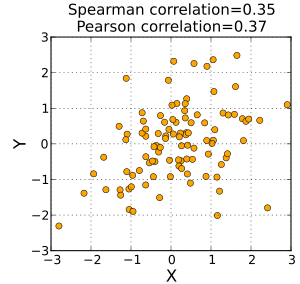
\includegraphics[scale=0.7]{images/spearman2.png}
\caption{When the data points are evenly spread,
both the Pearson's and the Spearman's
correlation coefficients will be low ( 0.35 and
0.37 respectively). Source:\cite{spearman2009Wiki}}
\label{fig:spearman2}
\end{figure}

\begin{figure}[h]
  \centering
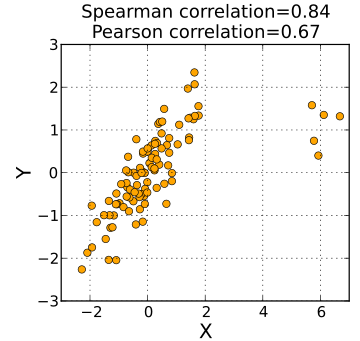
\includegraphics[scale=0.6]{images/spearman3.png}
\caption{Spearman's correlation coefficient is
more robust to outliers than Pearson's, because
it projects the data points to their ranks. As a result, Spearman's correlation
coefficient is much higher than Pearson's (0.84 vs 0.67)
Source:\cite{spearman2009Wiki}}
\label{fig:spearman3}
\end{figure}

The Spearman's rank correlation coefficient or Spearman's rho, named after
Charles Spearman, is a non-parametric estimator of the statistical dependence of
two random variables\cite{lehman2005jmp}. It intuitively measures how well
the dependence between two variables can be measured using a monotonic function.
It is normally computed in two steps:
\begin{enumerate}
 \item The ranks $ x_i, y_i $ of each of the data points in $X$ and $Y$ are
calculated.  
 \item The Spearman's rank correlation coefficient is computed by applying
Pearson's correlation coefficient on the previously computed ranks of the data
points\cite{myers2010research}.
\end{enumerate}

\rowcolors{1}{blue1}{blue2}

\begin{table}
  \centering
  Computing Spearman's ranks of the data points\\
  \begin{tabular}{ | c | c | c |}
    \hline
    \cellcolor{blue3} Variable $X_i$ & \cellcolor{blue3} Position in ascending
order & \cellcolor{blue3} Rank\\
    \hline
    0.3 & 1 & 1\\
    \hline
    0.6 & 2 & 2\\
    \hline
    1.2 & 4 & $ \frac{4+5}{2} $\\
    \hline
    1.2 & 5 & $ \frac{4+5}{2} $\\
    \hline
    0.8 & 3 & 3\\
    \hline
    1.9 & 6 & 1\\
    \hline
  \end{tabular}
  \caption{The data is initially sorted in ascending order. If the data point is
unique, then the rank is simply the position in the ordered list. Otherwise,
the rank is computed as the average of the positions of all the data points
with the same value.}
  \label{tab:ranks_table}
\end{table}

The calculation of the ranks is best illustrated in table \ref{tab:ranks_table}.
After the ranks $ x_i, y_i $ of each data point is calculated are calculated,
the Spearman's correlation coefficient is computed using the Pearson's
correlation coefficient as follows:

\begin{equation}
 r = \frac{\sum_{i=1}^{n}(x_i - \bar{x})(y_i -
\bar{y})}{\sqrt{\sum_{i=1}^{n}\left(x_i -
\bar{x}\right)^2}\sqrt{\sum_{i=1}^{n}\left(y_i -
\bar{y}\right)^2}} 
\end{equation}

Spearman's correlation coefficient is considered non-parametric in the sense
that one does not need to know any prior on the $X$ and $Y$ random variables, as
it does not require knowledge (i.e. the parameters) of the joint probability
distribution of $X$ and $Y$.

\subsection{Computing the GDV correlation matrix of a network}

We can use the Pearson's or Spearman's correlation coefficient previously
described to compute a GDV correlation matrix for a given network in the
following manner:
\begin{enumerate}
 \item We compute the Graphlet Distribution Vector (GDV) for every node in the
input network
 \item We then construct samples $ S_i, i\in {1,2,3, .. ,29} $
containing all the frequencies of the graphlet of type $i$ found in the GDVs of
the nodes.
 \item We compute the Pearson's (or Spearman's) correlation coefficient of each
pair of samples $ (S_i, S_j) $ and we put them in the 29x29 correlation matrix $
C_{ij} $.
\end{enumerate}

The newly obtained graphlet correlation matrix will be symmetric with respect to 
the main diagonal, as Pearson's correlation coefficient is also symmetric. In
order to display such a matrix, we can use a heat map, with blue representing -1
and red representing 1.

Given two matrices from two different networks $G$ and $H$, we can then calculate
the distance between them by performing pairwise-subtractions of the elements:

$$ D(G,H) = \sum_{i,j}\left(G(i,j) - H(i,j)\right)^2  $$

Note that the computed distance is always greater than 0. Using the distance,
the \emph{Graphlet Correlation Matrix Agreement} between $G$ and $H$ is
defined as: 

$$ Agreement = 1 - D(G,H) $$

One advantage of using such an Agreement based on Pearson's correlation
coefficient is that it has been shown to be more robust to noise in the network
data\cite{kuchaiev2009learning}.

\section{Canonical Correlation Analysis}

Canonical Correlation Analysis is a statistical method of analysing interdependence 
between two random variables $X$ and $Y$. The method was first introduced by 
Harold Hotelling in 1936\cite{hotelling1936relations} and it has been used for 
analysing and interpreting data in various fields including 
Psychology\cite{cooley1971multivariate}, Marketing\cite{fader1990cross} and 
Operations Research\cite{pisharodi1991interset}.

Given two random variables $X$ and $Y$ and a set of vector weights $a$ and $b$, 
let $u_1 = Xb_1$ and $u_2 = Xb_2$. Canonical Correlation Analysis (CCA) aims to 
find the weights $a$ and $b$ such that the correlation $ \rho = corr(t_1, u_1) $
is maximised. In this case, $u_1$ and $t_1$ are called the first canonical variates. 

The CCA process can be repeated again in order to find a second pair of canonical 
variates, with the additional condition that they are orthogonal to the first set 
of canonical variates. Thus, the second stage of the canonical correlation problem 
can be stated as follows:

Choose $a_2$,$b_2$ to maximise $r(t_2, u_2)$ such that $r(t_1, t_2) = 0$ and $r(t_2, t_2) = 0$ 

The number of "stages" to the canonical correlation problem depends on the number of variables. 
If $p$ is the number of $X$ variables and $q$ is the number of $Y$ variables, then the maximum 
number of canonical variates that can be computed is $min(p,q)$.

\subsection{Derivation of Canonical Correlation Analysis}

We first define the correlation matrix $R$ as:

\rowcolors{1}{white}{white}

$$R = 
\begin{pmatrix}
R_{YY} & R_{YX} \\
R_{XY} & R_{XX} 
\end{pmatrix}
$$

where $R_{XY}$ is the correlation matrix between $X$ and $Y$, while $R_{XX}$ and $R_{YY}$ are the correlation matrices of $X$ and $Y$.  


We find that solving the problem in  matrix form will in fact give the solution to all 
stages of the problem. Dropping the subscripts on $t$ and $u$, we restate the problem as follows:\\

Choose $a$, $b$ to maximise 

\begin{equation}
\label{cca_no_subscript}
r(t, u)=\frac{cov(t,u)}{\sqrt{var(t)var(u)}}
\end{equation}

The numerator of the objective function in equation (\ref{cca_no_subscript}) is simply given by:

$$Cov(t,u) = \frac{[t'u]}{n-1}=\frac{a'Y'Xb}{n-1} = a'R_{YX}b$$

By standardising $t$ and $u$, we effectively eliminate the denominator from the objective 
function in equation (\ref{cca_no_subscript}). Note that setting $ var(t) = 1 $ is equivalent to the following:
  
$$ var(t) = 1 $$
$$\implies \frac{[t't]}{n-1} = 1 $$
$$ \implies \frac{[a'Y'YA]}{n-1} = 1 $$
$$ \implies a'R_{YY}a = 1$$

Similarly, setting $var(u) = 1$ is the same as setting $b'R_{XX}b = 1$. Imposing these 
constraints, the problem becomes:\\

Choose $a$, $b$ to maximise $a'R_{XX}b$

subject to 

\begin{equation}
\label{cca_constraints}
a'R_{YY}a = 1 \text{ and } b'R_{XX}b = 1
\end{equation}

This constrained maximisation problem can be solved by using Lagrange multipliers and solving the first-order conditions. Using $\alpha/2$ and $\beta/2$ as Lagrange multipliers, the Lagrangian functions is then given by:

\begin{equation}
 L = a'R_{YX}b - \frac{\alpha}{2}(a'R_{YY}a - 1) - \frac{\beta}{2}(b'R_{XX}b - 1) 
\end{equation}

Differentiating with respect to $a$ and $b$ and setting the results equal to zero gives the first-order conditions:

\begin{equation}
\label{cca_foc1}
  \frac{\partial L}{\partial a} = 0 \implies R_{YX}b - \alpha R_{YY}a = 0
\end{equation}
\begin{equation}
\label{cca_foc2}
 \frac{\partial L}{\partial b} = 0 \implies R_{XY}a - \beta R_{XX}b = 0
\end{equation}

Taking the expression in equation (\ref{cca_foc1}) and pre-multiplying by $a'$ yields:

$$a'R_{YX}b - \alpha (a'R_{YY}a) = 0$$

which implies that $\alpha = r(t,u) $, the canonical correlation, because $a'R_{YY}a=1$ under the scaling constraints we have imposed for this problem. Similarly, taking equation (\ref{cca_foc2}) and pre-multiplying by $b'$ yields $\beta = r(t,u)$, which means that $\alpha = \beta$.

Now that the values of $\alpha$ and $\beta$ are known, we can substitute into equations (\ref{cca_foc1}) and (\ref{cca_foc2}) and solve the expressions for either $a$ or $b$.

Suppose we choose to solve for b. We use equation (\ref{cca_foc1}) to write $a$ as a function of $b$ as follows:

\begin{equation}
\label{cca_a}
  a = \frac{1}{r(t,u)}R^{-1}_{YY}R_{YX}b
\end{equation}

We then substitute the right-hand side of equation (\ref{cca_a}) above for $a$ in equation (\ref{cca_foc2}) and solve for $b$. The result is:

\begin{equation}
 R_{XY}\left( \frac{1}{r(t,u)}R^{-1}_{YY}R_{YX}b \right) = r(t,u)R_{XX}b
\end{equation}

Premultiplying by $R^{-1}_{XX}$ and mutiplying through by $r(t,u)$ gives:

\begin{equation}
  \label{cca_eigen_eq}
 [R^{-1}_{XX}R_{XY}R^{-1}_{YY}R_{YX}]b = r^2(t,u)b
\end{equation}

Equation (\ref{cca_eigen_eq}) is an eigenvector-eigenvalue problem. The vector $b$ is the first eigenvector of the matrix $R^{-1}_{XX}R_{XY}R^{-1}_{YY}R_{YX}$. The proportionality constant, which is the eigenvalue corresponding to b, is the squared canonical correlation $r^2(t,u)$. Although we will not prove this in the report, the structure of the canonical correlation problem ensures that the eigenvalues are both real and non-negative\cite{carroll1997mathematical}. 

We can now find $a$ by substituting $b$ into equation (\ref{cca_a}). We also find that a is the first eigenvector of the matrix $R^{-1}_{YY}R_{YX}R^{-1}_{XX}R_{XY}$. The first eigenvalue is again the squared canonical correlation.

\subsection{Canonical Loadings}

To facilitate interpretation, it is helpful to look at the canonical loadings, which are the correlations between original variables and the canonical variates. The correlations between $X$ and $u$, which we denote $f$, are given by:

\begin{equation}
 f = \frac{1}{n-1}X'u = \frac{1}{n-1}X'(Xb) = R_{XX}b
\end{equation}

Similarly, the correlations between $Y$ and $t$, denoted $g$ are given by:

\begin{equation}
 g = \frac{1}{n-1}Y't = \frac{1}{n-1}Y'(Ya) = R_{YY}a
\end{equation}

\subsection{Canonical Cross-Loadings}